% slide template
\begin{frame}
  \frametitle{Canonical discriminant plots for MANOVA}
  \begin{itemize}
	\item HE plots show the variation in means relative to error for 2 selected variables
	\item All bivariate relations can be shown in an HE plot matrix
	\item Alternatively, as in the biplot, we can project the data into a low-rank (2D) space
      \begin{itemize*}
	  \item CDA plot shows observations in the 2D space that maximally discriminates among groups
	  \item The canonical variates are linear combinations of $\mat{Y} = (\vec{y}_1 , \vec{y}_2, \dots , \vec{y}_p )$
	  with weights given by the latent vectors of $\mat{H} \mat{E}^{-1}$
	  \item Vectors from the origin (grand mean) for the observed variables show the correlations with the canonical dimensions
	  \end{itemize*}
	\item Properties:
      \begin{itemize*}
	  \item Canonical variates are uncorrelated
	  \item Circles of radius \(\sqrt { \chi_2^2 ( 1 -\alpha  ) /  n_i }\) give confidence regions for group means.
	  \item Variable vectors show how variables discriminate among groups
	  \item Lengths of variable vectors $\sim$ contribution to discrimination
	  \end{itemize*}
  \end{itemize}
\end{frame}

\begin{frame}
  \frametitle{CDA Examples: Pottery data}

\begin{center}
  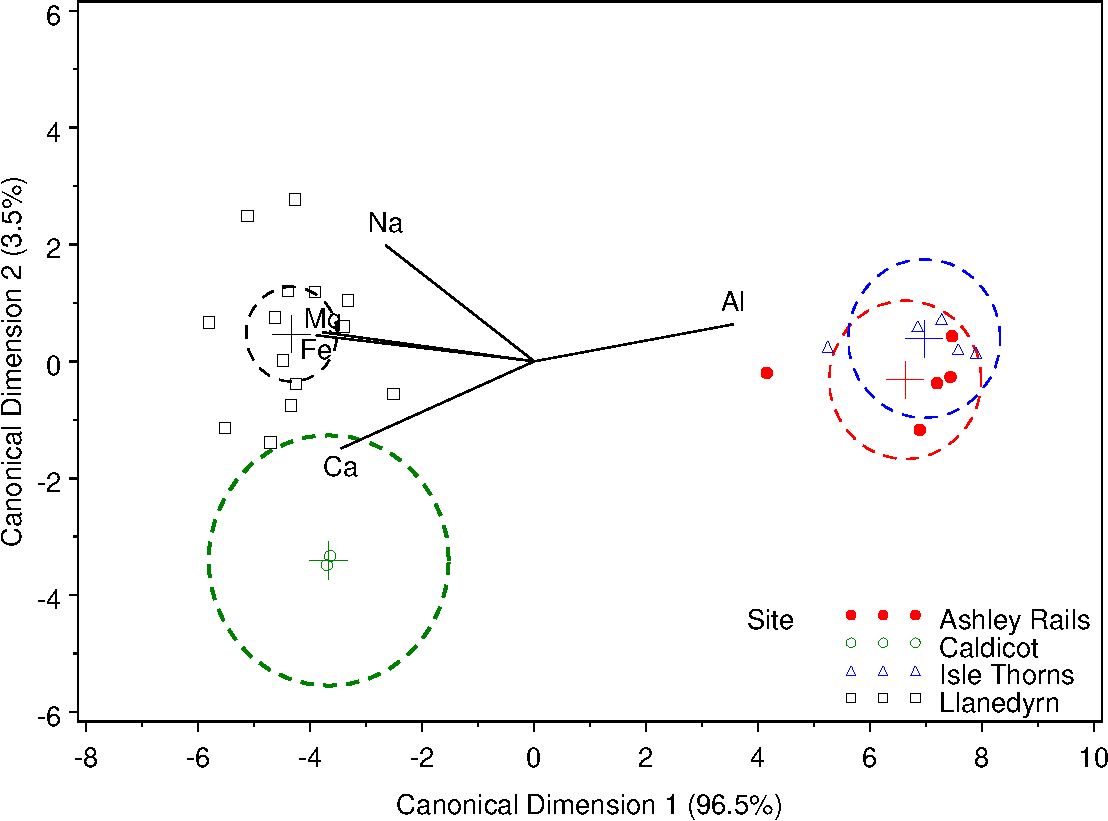
\includegraphics[width=.85\textwidth,clip]{fig/pottery-can}
  \\ Canonical discriminant plot for pottery data
\end{center}

\end{frame}

\begin{frame}
  \frametitle{CDA Examples: Iris data}
\begin{center}
  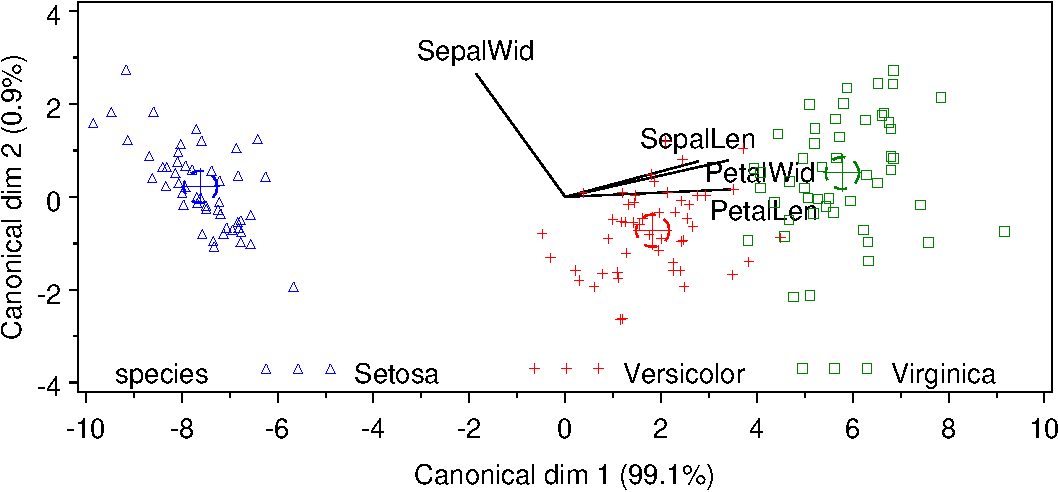
\includegraphics[width=.85\textwidth,clip]{fig/gcaniris}
  \\ Canonical discriminant plot for iris data
\end{center}

\end{frame}

\begin{frame}
  \frametitle{CDA Examples: Baseball data, by player position}
\begin{center}
  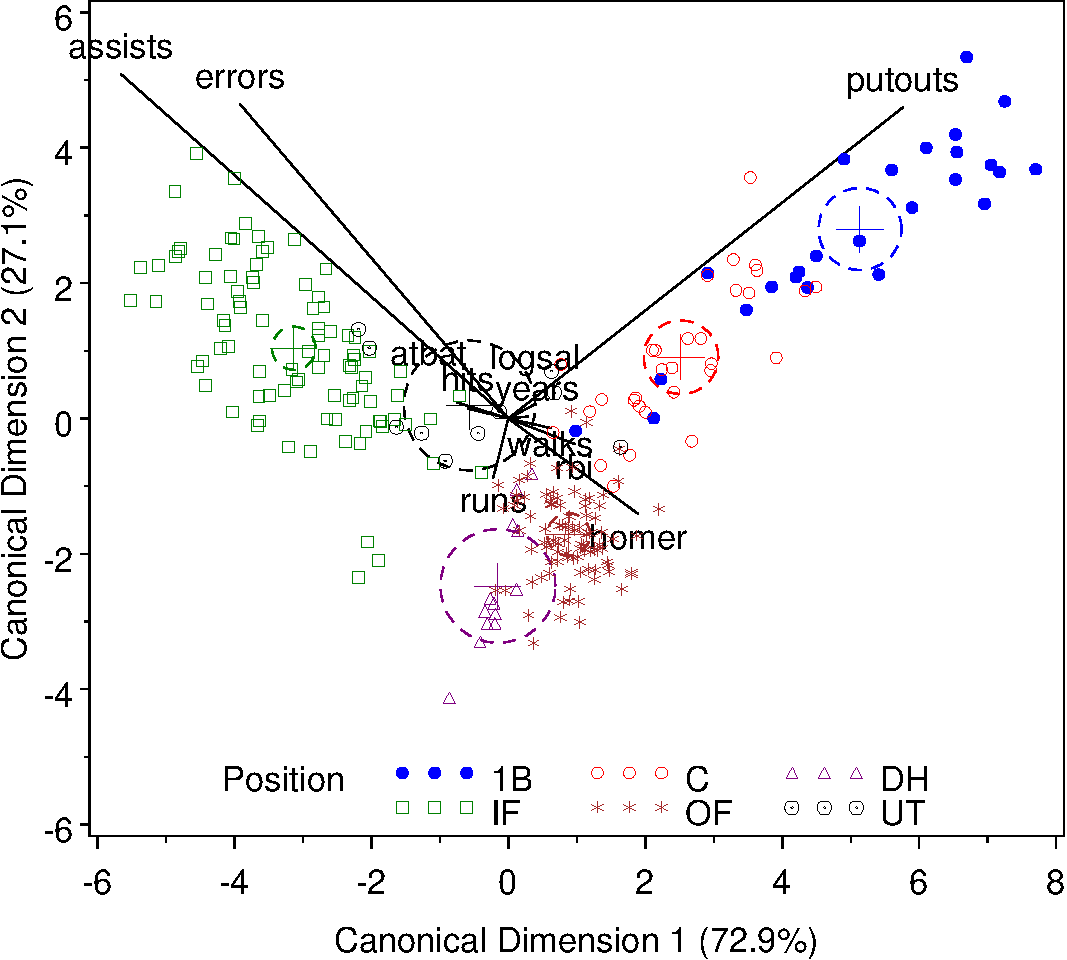
\includegraphics[width=.75\textwidth,clip]{fig/gcanbase}
%  \\ Canonical discriminant plot, by player position
\end{center}

\end{frame}

\begin{frame}
  \frametitle{Canonical correlation plots for MMRA}
  \begin{itemize}
	\item HE plots show the relations of predictors to 2 selected response variables
	\item All bivariate relations can be shown in an HE plot matrix
	\item Alternatively, plot the data and variable vectors in 2D space of largest canonical correlations.
      \begin{itemize*}
	  \item Two plots: standardized canonical scores
	  \item Responses plot: $\vec{u}_1 = \vec{a}_1\trans \mat{Y}$ and $\vec{u}_2 = \vec{a}_2\trans \mat{Y}$
	  \item Predictors plot: $\vec{v}_1 = \vec{b}_1\trans \mat{X}$ and $\vec{v}_2 = \vec{b}_2\trans \mat{X}$
	  \item Vectors from the origin (grand mean) for the observed variables show the correlations with the canonical dimensions
	  \end{itemize*}
	\item Properties:
      \begin{itemize*}
	  \item Canonical variates are uncorrelated: data ellipses are circular
	  \item Variable vectors show how predictors are related to response variables
	  \item Lengths of variable vectors $\sim$ contribution to between-set correlations
	  \end{itemize*}
  \end{itemize}

\end{frame}

\begin{frame}
  \frametitle{Cancorr Example: Rower's data}

\begin{center}
 \begin{minipage}[c]{.49\linewidth}
  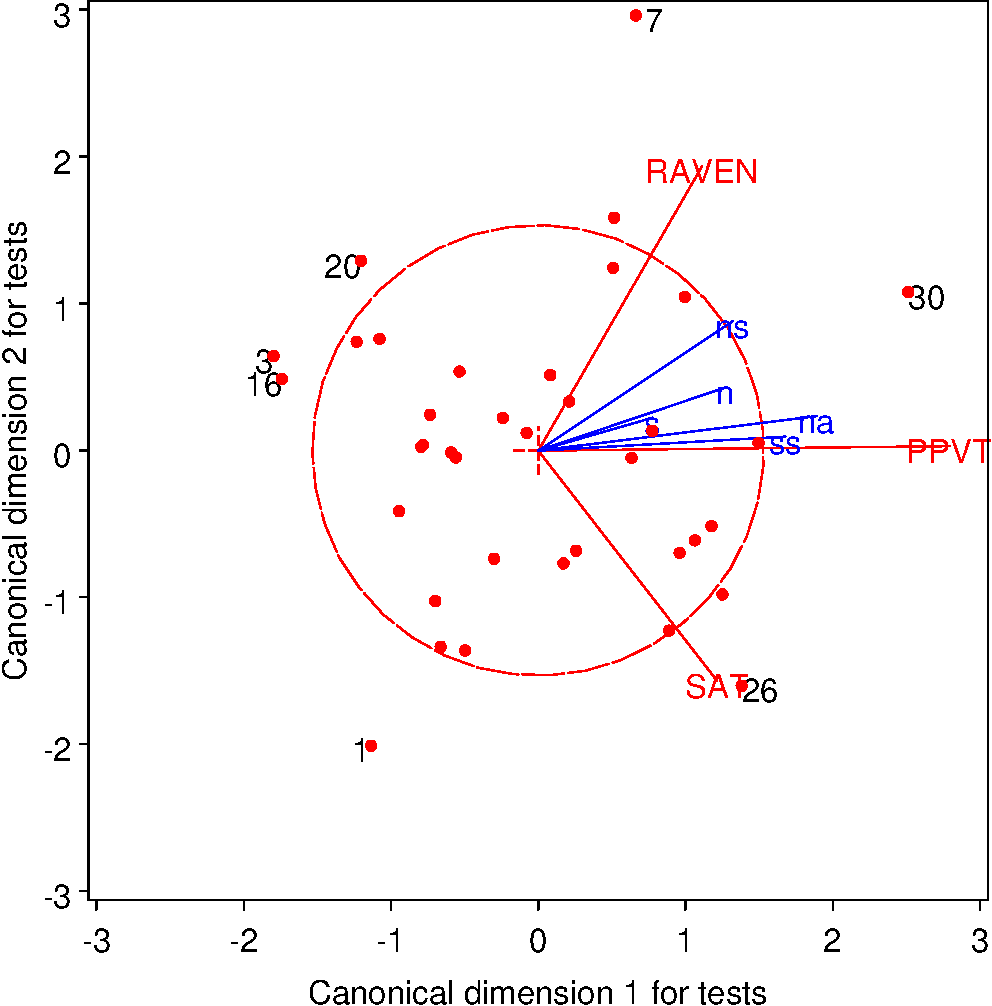
\includegraphics[width=1\linewidth,clip]{fig/canppvt11}
 \end{minipage}%
 \hfill
 \begin{minipage}[c]{.49\linewidth}
  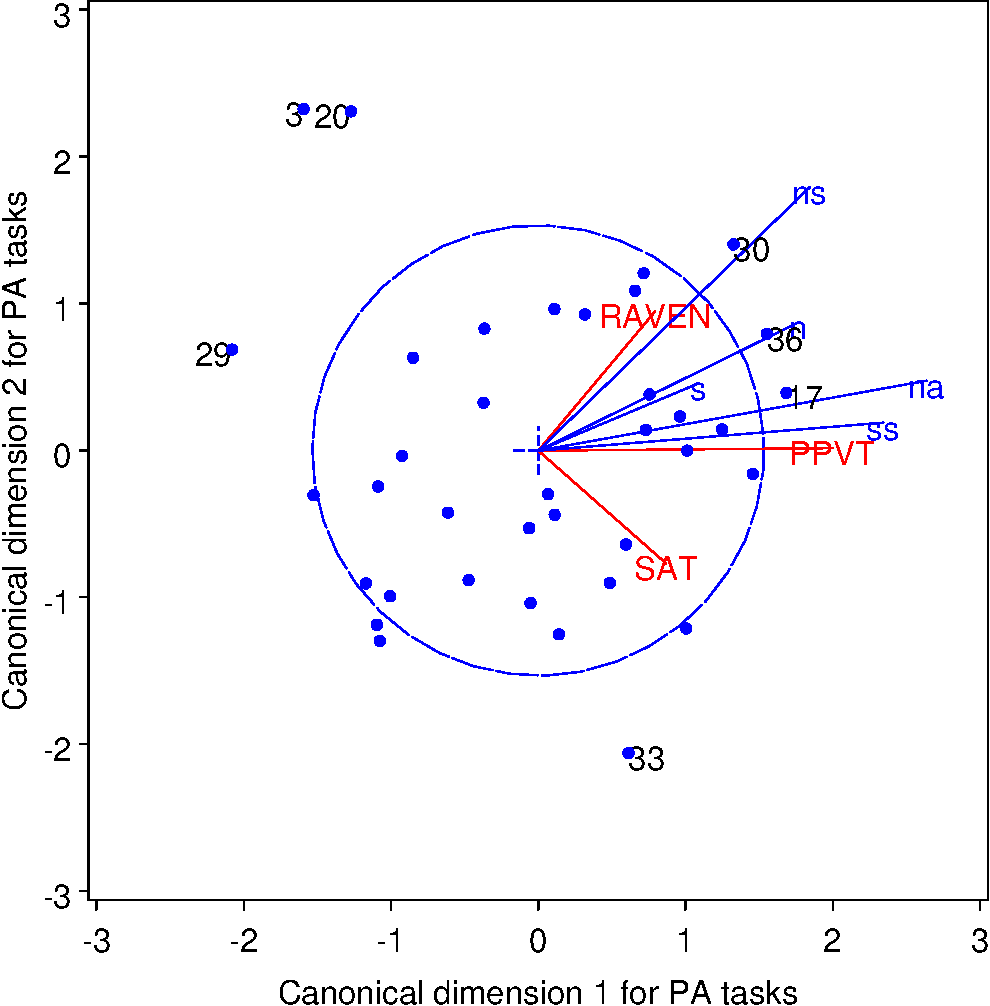
\includegraphics[width=1\linewidth,clip]{fig/canppvt12}
 \end{minipage}
 \\ Can. dim 1:  $\rho_1 = 0.72$:  PPVT $\longleftrightarrow$ NA, SS tasks
 \\ Can. dim 2:  $\rho_2 = 0.49$:  RAVEN, SAT $\longleftrightarrow$ NS task
 \end{center}

\end{frame}
